\documentclass[../resume.tex]{subfiles}

\begin{document}

\section{Graduate Research}

\subsection{Neuron Theory and Simulations}

\subsubsection{Spike-Triggered Descent}
I developed a technique in python to classify the function a network of neurons compute with respect to a signal.  Here's the abstract, an equation, and a figure from our \href{https://arxiv.org/pdf/2005.05572.pdf}{paper}.

The characterization of neural responses to sensory stimuli is a central problem
in neuroscience. Spike-triggered average (STA), an influential technique, has been
used to extract optimal linear kernels in a variety of animal subjects. However,
when the model assumptions are not met, it can lead to misleading and imprecise
results. We introduce a technique, called spike-triggered descent (STD), which can
be used alone or in conjunction with STA to increase precision and yield success
in scenarios where STA fails. STD works by simulating a model neuron that learns
to reproduce the observed spike train. Learning is achieved via parameter optimization that relies on a metric induced on the space of spike trains modeled as a
novel inner product space. This technique can precisely learn higher order kernels
using limited data. Kernels extracted from a \textit{Locusta migratoria} tympanal nerve
dataset demonstrate the strength of this approach.

\begin{equation} \label{eq:GCSRMdt}
\resizebox{.9\hsize}{!}{$
\Delta t_l^O = 
\frac{
\sum \frac{\partial \eta}{\partial t} \big|_{t_l^O - t_k^O}  \Delta t_k^O
-
\sum \frac{\partial \eta}{\partial \mu} \big|_{t_l^O - t_k^O} \Delta \mu_k
-
\Delta K_0
- 
\sum_{n=1}^N  \idotsint_n
(\sum B_i(\tau_{1 \rightarrow n}) \Delta \beta_{i,l})
\prod_{j = 1}^n
x(t_l^O - \tau_j)
d\tau_j
}
{
\sum_{n=1}^N  \idotsint_n
K(\tau_{1 \rightarrow n}; \beta_{i,l})
\Big[
\sum_{m=1}^n
\Big[ 
\prod_{j \ne m}^n
x(t_l^O - \tau_j)
\Big]
\frac{\partial x}{\partial t} \big|_{t_l^O - \tau_m} 
\Big]
\prod_{j = 1}^n
d\tau_j
+ \sum \frac{\partial \eta}{\partial t} \big|_{t_l^O - t_k^O}
}
$}
\end{equation}

%https://tex.stackexchange.com/questions/25414/how-to-create-magnified-subfigures-and-corresponding-boxes-for-portions-of-a-lar
\begin{figure}[ht]\centering
\begin{tikzpicture}[
    zoomboxarray,
    zoomboxarray columns=3,
    zoomboxarray rows=1,
%    connect zoomboxes,
    zoombox paths/.append style={line width=3pt}
]
    \node [image node] { 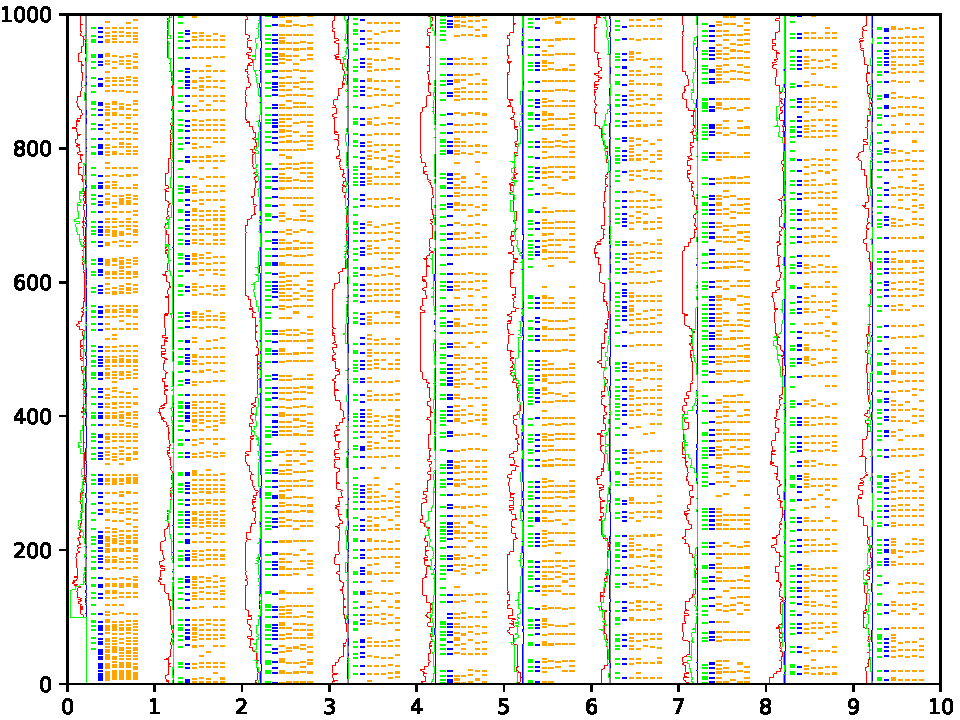
\includegraphics[width=0.45\textwidth]{E_spikes_100ms_a2a_grid_visableMarkers.pdf} };
    \zoombox[magnification=4, color code=lime]{2*0.0911 + 0.108 , 7*0.075 + 0.18}
    \zoombox[magnification=4, color code=blue]{4*0.0911 + 0.108 , 4*0.075 + 0.18}
    \zoombox[magnification=4, color code=orange]{8*0.0911 + 0.108 , 3*0.075 + 0.18}
%    \zoombox[magnification=6, color code=purple]{3*0.0911 + 0.115 , 6*0.084 + 0.135}
%    \zoombox[magnification=6, color code=yellow]{8*0.0911 + 0.115 , 1*0.084 + 0.135}
\end{tikzpicture}
\end{figure}

\subsection{Medical Imaging}
I created an interactive volume calculation tool for neurosurgeons to diagnose hydrocephalus and create a medical atlas.  I implemented this in python with pygame, numpy, scipy, and skimage.  There are a variety of features and multiple configurable methods of classification.  The following image shows an example of the application automatically measuring the volume of a ventricle region with one click (red circle).  The cursor (blue circle) is show along with a zoomed in area around it.  There are 25 separate controls allowing a variety of usability.

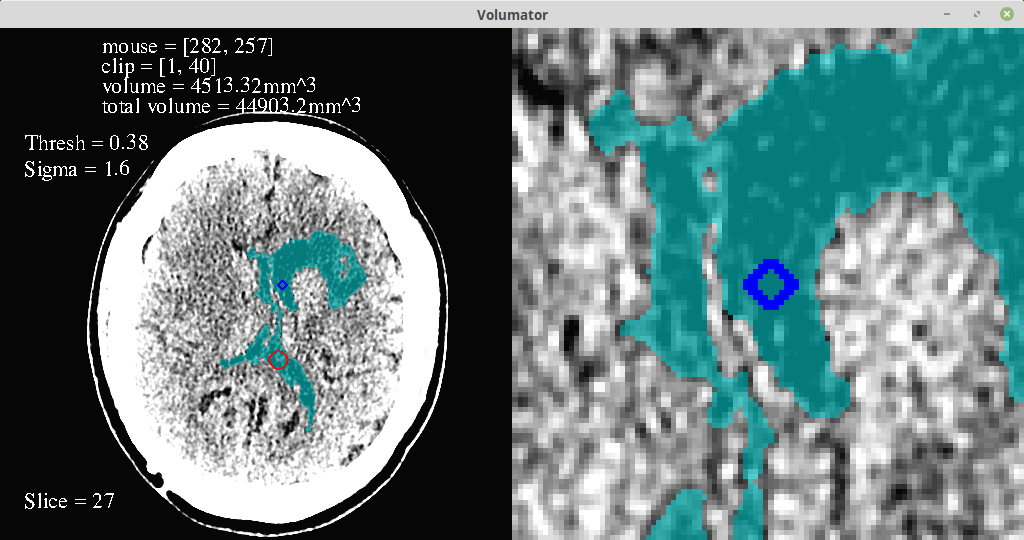
\includegraphics[scale=0.3]{../research/volumator.png} 

\subsection{Computational Genetics}
Worked with a computational genetics lab to increase the training accuracy on the assembly of rAAV codon mutations.  Assisted in improving the classification accuracy from $\sim 75\%$ to $\sim 99.5\%$.  Using a mixture of python and bash scripting I created many graphs like the following to explore the mutation space.

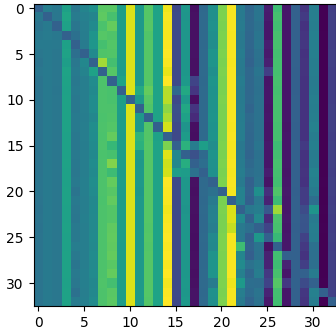
\includegraphics[scale=0.5]{../research/sum_modes_RAmRU.png} 

\subsection{Landmine Detection}

I worked on classifying underground objects with recorded from ground penetrating radar.  The aim of this project was to explore the effectiveness of using Deep Belief Networks to detect landmines.  We used a mixture of python, theano, pytorch, keras, scikit learn, and octave.  The following ROC curve shows the true and false positive rates for various objects.

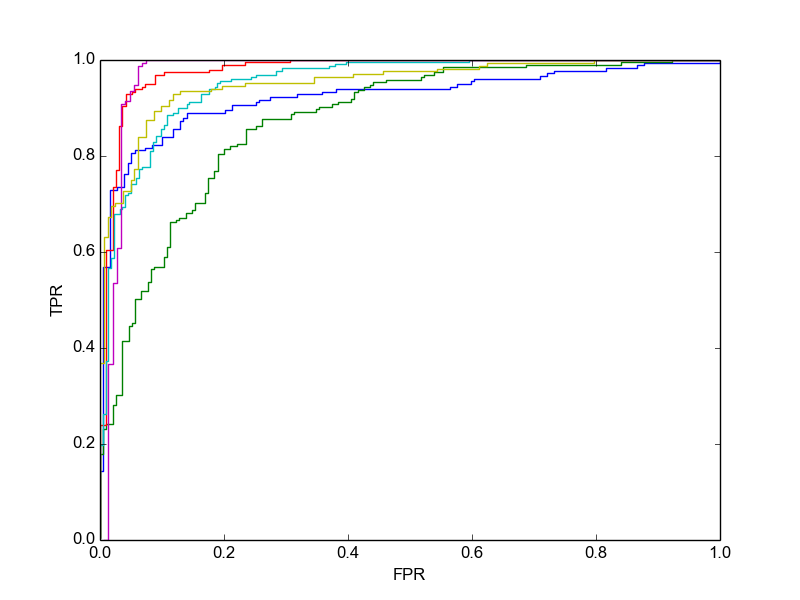
\includegraphics[scale=0.5]{../research/roc.png}

\section{Undergraduate Research}

\subsection{Optics Lab}
Machined optics equipment and set up equipment for analysis with a multi omnidirectional spectrometer (MONSTR) to conduct fourier transform infrared spectroscopy (FTIR).

\subsection{Nanotech Lab}
Conducted carbon vapor deposition experiments to synthesize graphene nanoribbons and boron doped carbon nanotubes.  Characterized these materials with an assortment of SEM, TEM, PPMS, XRD, EDX, and Raman. 

\subsection{Computational Biophysics Lab}
I worked on a project to simulate collagen elasticity from the ground up using pdb files with unix commands and Gromacs in order to match experimental results.


\end{document}